\documentclass{mini}
\usepackage[utf8]{inputenc}
%------------------------------------------------------------------------------%
\title{IFS - iterated function systems}
\author{Marta Sommer}
\supervisor{dr Agnieszka Badeńska}
\type{licencjac}
\discipline{matematyka}
\monthyear{wrzesień 2013}
\date{\today}
\album{237503}
%------------------------------------------------------------------------------%
\usepackage{color}

%-----------------------------new envirenmenty---------------------------------------------------------
\begin{document}
\maketitle
\tableofcontents

\newtheorem{tw}{Twierdzenie}[chapter]

\newenvironment{dow1}{\textbf{\textit{Dowód pierwszy}}}{\begin{flushright} $\blacksquare$ \end{flushright}} 

\newenvironment{dow2}{\textbf{\textit{Dowód drugi}}}{\begin{flushright} $\blacksquare$ \end{flushright}}

\newtheorem{df}{Definicja}[chapter]

\newenvironment{dow}{\textbf{\textit{Dowód}}}{\begin{flushright} $\blacksquare$ \end{flushright}}

%---------------------------------------------------------------------------------------------------




\chapter*{Wstęp}


Do wyjaśnienia własności iterowanych systemów funkcyjnych potrzebna jest definicja wymiaru Hausdorffa. Spróbuję ją więc w tym rozdziale wprowadzić i wyjaśnić.



%------------------------------wymiar hausdorffa-----------------------------------------------
\chapter{Wymiar Hausdorffa}


\begin{df}

Niech $A$ - dowolny podzbiór $\mathbb{R}^n$, ustalmy $s>0$. Weźmy pod uwagę dowolne przeliczalne pokrycie $A$ tzn. zbiory $U_1,U_2,\ldots\subset\mathbb{R}^{n}$ takie, że $A\subset\bigcup_{i=1}^{\infty}{U_i}$, $\delta>0$.
Wtedy miarą zewnętrzną Hausdorffa zbioru $A$ nazywamy:

\begin{equation}\label{mzh}
\mathcal{H}^{s}_{\delta}{(A)} = inf \sum^{\infty}_{i=1}{(diam U_i)^{s}}\textrm{,}
\end{equation}

gdzie $diam$ - średnica zbioru, a infimum jest wzięte po wszystkich takich pokryciach $\lbrace U_i\rbrace^{\infty}_{i=1}$ zbioru $A$, że $ diam U_i < \delta$ dla każdego $U_i$.  

\end{df}

\begin{df}

Miarą Hausdorffa zbioru $A$ nazywamy:

\begin{equation}
\mathcal{H}^s(A)=lim_{\delta\rightarrow0^+} \mathcal{H}^s_{\delta}(A)
\end{equation}

\end{df}


\vspace*{2\baselineskip}

Granica z powyższej definicji istnieje dla każdego $F \subset \mathbb{R}^n$, gdyż $\mathcal{H}^{s}_{\delta}$ jest niemalejącą funkcją $\delta$. Wynika to z tego, że zmniejszając $\delta$ zawężamy klasę dopuszczalnych pokryć, po których brane jest infimum.

\vspace*{1\baselineskip}

Okazuje się, że istnieje taka liczba $t\geqslant0$, że:

\begin{eqnarray}
\forall_{s<t}\hspace{5mm} \mathcal{H}^s(A)&=&+\infty \\
\forall_{s>t} \hspace{5mm}\mathcal{H}^s(A)&=&0 
\end{eqnarray}

Wtedy liczbę $t$ nazywamy wymiarem Hausdorffa zbioru $A$ i oznaczamy $dim_H(A)$.

Skąd jednak wiemy, że taka liczba istnieje? Przedstawię poniżej krótkie wyprowadzenie tego faktu.

Rozważmy równianie \eqref{mzh}. Łatwo widać, że dla dowolnego zbioru $F\subset \mathbb{R}^n$ i $\delta <1$, $\mathcal{H}^s_{\delta}(F)$ jest nierosnącą funkcją $s$. Wynika z tego, że $\mathcal{H}^s$ również jest nierosnącą funkcją $s$. Tak naprawdę prawdą jest jeszcze więcej. Otóż, jeśli $s<t$ i $\lbrace U_i \rbrace$ jest $\delta$-pokryciem $F$, to:

$$ \sum_i |U_i|^t = \sum_i |U_i|^{t-s}|U_i|^s \leqslant \delta^{t-s}\sum_i |U_i|^s$$

Zatem, biorąc infimum po pokryciach, otrzymujemy, że $\mathcal{H}^t_{\delta}(F)\leqslant \delta^{t-s} \mathcal{H}^s_{\delta}(F)$. Gdy $\delta\rightarrow 0$ oraz $\mathcal{H}^s(F)<\infty$, to $\mathcal{H}^t(F)=0$ dla $t>s$. 


Bardziej formalnie można to zapisać jako:

\begin{equation}
dim_H(A)= \inf\lbrace s: \mathcal{H}^s(A)=0\rbrace=\sup\lbrace s: \mathcal{H}^s(A)=\infty\rbrace
\end{equation}
%--------------------------------------tw pomocnicze----------------------------------------

\chapter{Twierdzenia pomocnicze}

%-------------------------------------tw mass distribution -------------------------------------

\begin{tw}{\textit{(Mass distribution principle)}}\label{mass}

Niech $\mu$ będzie miarą na $F$ i przypuśćmy, że dla pewnego $s$ istnieją $c>0$ i $\delta>0$ takie, że:

\begin{equation}
\forall_{U \hspace{1mm}\textrm{takiego, że} \hspace{1mm} |U|\leqslant \delta} \hspace{5mm} \mu (U) \leqslant c|U|^s
\end{equation}   

Wtedy $\mathcal{H}^s(F)\geqslant \frac{1}{c} \mu (F)$ oraz $s \leqslant dim_{H}F \leqslant \underline{dim_BF} \leqslant \overline{dim_BF}$

\end{tw}

%------------------------------------dowód mass distribution

\begin{dow}

Niech $U_i$ - dowolne pokrycie $F$. Widzimy wtedy, że:

$ 0 \leq \mu (F) \leqslant \mu( \bigcup_i U_i ) \leqslant \sum_i \mu (U_i) \leqslant \sum_i c|U_i|^s = c \sum_i |U_i|^s $

A zatem: 

$ \sum_i |U_i|^s \geqslant \frac{\mu(F)}{c} $

Bierzemy infimum po wszystkich pokryciach:

$ \inf \sum_i |U_i|^s \geqslant \frac{\mu(F)}{c} $

$ \mathcal{H}^s_{\delta} (F) \geqslant \frac{1}{c} \mu (F) $

Czyli przy $ \delta \rightarrow 0^+ $:

$ \mathcal{H}^s (F) \geqslant \frac{1}{c} \mu (F) $

A skoro $ \mu(F)>0 $, to $dim_HF \geqslant s$. 

\end{dow}

%----------------------------------tw o jabłkach w koszyku--------------------------------

\begin{tw}{\textit{(O jabłkach w koszyku)}}\label{apple}

Niech $\lbrace V_i \rbrace$ będzie rodziną rozłącznych i otwartych podzbiorów $\mathbb{R}^n$ takich, że każdy $V_i$ zawiera kulę o promieniu $a_1r$ i jest zawarty w kuli o promieniu $a_2r$, gdzie $a_1, a_2>0$ i $r>0$.

Wtedy dowolna kula $B$ o promieniu $r$ przecina co najwyżej $(1+2a_2)^n a_1^{-n}$ domknięć $\overline{V_i}$.

\end{tw}

%-------------------------------------dow o jabłkach w koszyku---------------------------------------

\begin{dow}

Jeśli $\overline{V_i}$ przecina $B$, wtedy $\overline{V_i}$ jest zawarte w kuli współśrodkowej z $B$ o promieniu $(1+2a_2)r$. Wynika to z prostego rachunku: 

$r+2a_2r = r(1+2a_2)$

Przypuśćmy, że $q$ zbiorów $\overline{V_i}$ przecina $B$. Wtedy, sumując objętości odpowiednich wewnętrznych kul o promieniach $a_1r$, otrzymujemy:

$q(a_1r)^n \leqslant (1+2a_2)^nr^n$

Czyli: $q \leqslant (1+2a_2)^n a_1^{-n}$
 
\end{dow}

%-------------------------------tw banacha o pkt stalym-------------------------------------

\begin{tw}{\textit{(Banacha o punkcie stałym)}}\label{banach}

Niech $(X,\rho)$ będzie przestrzenią metryczną zupełną a funkcja $f: X\longrightarrow X$ kontrakcją. Wtedy:
\begin{enumerate}
\item f ma dokładnie jeden punkt stały $x_0$, tzn. $\exists !_{x_0} \hspace{5mm}f(x_0)=x_0$
\item Dla każdego $x \in X$ ciąg $(x,f(x,f(f(x))),\ldots)$ jest zbieżny do $x_0$.
\end{enumerate}

\end{tw}

\chapter{Twierdzenie o istnieniu atraktora}

%-------------------------- tw o istnieniu atraktora -------------------------------------


\begin{tw}

Rozważmy iterowany układ funkcyjny (IFS) określony na zbiorze 
$D \subset \mathbb{R}^{n}$ 
kontrakcjami 
$ \lbrace S_1, \ldots,S_m \rbrace $ 
tzn. funkcjami takimi, że 
$S_i: \hspace{2mm} D \longrightarrow D$ 
oraz

\begin{equation}
\forall_{x,y\in D} \hspace{2mm} \forall_{i=1,\ldots ,m} \hspace{5mm} \vert S_i(x)-S_i(y) \vert \leq c_i \vert x-y \vert, 
\end{equation}

gdzie $ c_i < 1 $.

Wtedy istnieje jednoznacznie wyznaczony atraktor $F$, tj. niepusty i zwarty zbiór taki, że:

\begin{equation}\label{d1}
F = \bigcup^{m}_{i=1}{S_i(F)} 
\end{equation}

Jeśli dodatkowo zdefiniujemy przekształcenie $S$ na klasie $X$ niepustych i zwartych podzbiorów $D$ jako:

\begin{equation}\label{d3}
\forall_{E \in X} \hspace{5mm} S(E) = \bigcup^{m}_{i=1} S_i(E)
\end{equation}

oraz oznaczymy przez $S^k$ - k-tą iterację $S$ tzn. 

$ S^0(E) = E $,

$ S^k(E) = S(S^{k-1}(E)) \hspace{4mm}\textrm{dla} \hspace{2mm} k \geq 1 \textrm{.}$

Wtedy:

\begin{equation}\label{d2}
\forall_{E \in X \hspace{2mm} \textrm{takiego, że} \hspace{2mm} \forall_{i=1,\ldots ,m} \hspace{2mm} S_i(E) \subset E} \hspace{5mm} F = \bigcap^{\infty}_{k=0} S^k(E)
\end{equation}

\end{tw}


%--------------------------dowód 1 o istn atraktora ---------------------------------------------------

 


\begin{dow1}

Zauważmy, że $S$ przekształca zbiory z $X$ na zbiory z $X$.
Do dowodu wykorzystamy poniższe twierdzenie.

\begin{tw}\label{tp1}

Przekształcenie 
$S=\bigcup^{m}_{i=1} S_i \textrm{:} \hspace{2mm} X\longrightarrow X$
jest kontrakcją w metryce Hausdorffa, jeśli wszystkie przekształcenia
$S_1,\ldots ,S_m$: $D \longrightarrow D$
są kontrakcjami.

\end{tw}

\begin{dow}

Niech $S_1,\ldots ,S_m$ - kontrakcje.

Zatem istnieje liczba $c<1$ ($c=\max_{1\leqslant i\leqslant m}{c_i}$) taka, że:

$$ \forall_{p,q \in D} \hspace{2mm} \forall_{i=1,\ldots ,m} \hspace{5mm} \vert S_i(p)-S_i(q)\vert \leqslant \vert p-q \vert $$

Niech $A,B \in X$. Wtedy:

$$ \forall_{p \in A} \hspace{2mm} \exists_{q \in B} \hspace{5mm} \vert p-q \vert \leqslant d(A,B) \textrm{,}$$

gdzie $d$ - metryka Hausdorffa. Oznaczmy $d(A,B)$ jako $\delta$.

Zatem:

$$\forall_{i=1,\ldots ,m} \hspace{5mm} \vert S_i(p)-S_i(q) \vert \leqslant c \vert p-q \vert \leqslant cd(A,B)=c\delta$$

Czyli $S_i(A) \subset (S_i(B))_{c\delta}$.

Stąd 
$ \hspace{2mm} S(A)=\bigcup^{m}_{i=1} S_i(A) \subset \bigcup^{m}_{i=1} (S_i(B))_{c\delta} = (\bigcup^{m}_{i=1} S_i(B))_{c\delta} = (S(B))_{c\delta}  $.

Analogicznie 
$S(B) \subset (S(A))_{c\delta}$.

Czyli $d(S(A),S(B))\leqslant c\delta = cd(A,B)$.

\end{dow}

Wróćmy teraz do dowodu naszego twierdzenia.

Wiemy zatem, że $S$ jest kontrakcją na $(X,d)$.

Można pokazać, że $d$ jest zupełną metryką na $X$.
Spełnione są więc założenia tw. Banacha o punkcie stałym - tw. \eqref{banach}.
Zatem, jako wniosek z tego twierdzenia, otrzymujemy, że $S$ ma jednoznacznie wyznaczony punkt stały $F$. Czyli $S(F)=F$, co dowodzi \eqref{d1}.

Co więcej, $S^k(E)\longrightarrow F$, gdy $k\longrightarrow\infty$. W szczególności, jeśli $S_i(E) \subset E$ dla każdego $i$, wtedy $S(E) \subset E$ i $\lbrace S^k(E)\rbrace^{\infty}_{k=1}$ jest zstępującą rodziną zbiorów niepustych i zwartych. Czyli $F = \bigcap^{\infty}_{k=0} S^k(E)$, co dowodzi \eqref{d2}.

\end{dow1}

%-----------------------------------dowód2 o istn atraktora-------------------------------------

  

\begin{dow2}

Niech $E \in X$ będzie zbiorem takim, że $S_i(E) \subset E$ dla każdego $i=1,\ldots ,m$.
Taki zbiór istnieje. Weźmy na przykład $E=D \cap \overline{B}(0,r)$ dla odpowiednio dużego $r>0$, gdzie $\overline{B}(0,r)$ oznacza kulę domkniętą o promieniu $r$ i środku w $0$.
Uzasadnię, że nasz zbiór $E$ spełnia żądany warunek.

Wiemy, że $S_i(D) \subset D$ (z definicji $S_i$). Jeśli znajdziemy takie $r>0$, dla którego $S_i(\overline{B}(0,r)) \subset \overline{B}(0,r)$, wtedy będziemy mieć, że $S_i(D \cap \overline{B}(0,r)) \subset D \cap \overline{B}(0,r)$.

Niech $x \in \mathbb{R}^n$, $y \in \mathbb{R}^n$.

$S_i(x)=c_ix + y_i$

Zatem,

$S_i(\overline{B}(0,r))=\overline{B}(y_i,c_ir) \subset \overline{B}(0,r)$

$r$ szacujemy więc w następujący sposób:

$r> \vert y \vert + c_ir$

$r(1-c_i)>\vert y \vert$

$r>\frac{\vert y \vert}{1-c_i}$, bo $c_i<1$

Zatem dla odpowiednio dużego $r$ wybrane $E$ spełnia warunek $S_i(E) \subset E$.

Wtedy $S^k(E) \subset S^{k-1}(E)$.

Czyli $\lbrace S^k(E) \rbrace^{\infty}_{k=0}$ jest zstępującą rodziną zbiorów niepustych i zwartych (bo $E$ jest domknięty - jako domknięcie zbiorów domkniętych - i ograniczony), czyli istnieje niepuste i zwarte przecięcie $F = \bigcap^{\infty}_{k=0} S^k(E)$. Wynika to z twierdzenia, że zstępująca rodzina zbiorów domkniętych ma domknięte przecięcie.

Wtedy:

\mbox{$S(F)=S(\bigcap^{\infty}_{k=0} S^k(E))=\bigcap^{\infty}_{k=0} S(S^k(E))=\bigcap^{\infty}_{k=0} S^{k+1}(E)=\bigcap^{\infty}_{n=1} S^n(E)=\bigcap^{\infty}_{n=0} S^n(E)=F$}

Czyli $F$ spełnia \eqref{d3}, czyli jest atraktorem IFS. Ale czy wyznaczonym jednoznacznie?

Niech $A,B$ - atraktory IFS. Zatem:

$S(A)=A$ oraz $S(B)=B$.

Ponieważ $S$ jest kontrakcją ze stałą $c=\max_{1\leqslant i\leqslant m}{c_i}$, $0<c<1$, patrz  (tw.~ \ref{tp1}), więc:

$d(S(A),S(B))\leqslant cd(A,B)$

$d(A,B) \leqslant cd(A,B)$

$d(A,B)-cd(A,B)\leqslant 0$

$d(A,B)(1-c)\leqslant0$

$d(A,B)\leqslant 0 \Longrightarrow d(A,B)=0 \vee c\leqslant1$, co jest sprzeczne z założeniem.

Zatem $d(A,B)=0$. A z definicji metryki wiemy, że wtedy $A=B$.
\end{dow2}



\chapter{Twierdzenie o wymiarze fraktali}

%---------------------------------------def open set condition-----------------------------------

\begin{df}\label{osc}

Funkcje $S_1,\ldots,S_m$ takie, że $S_i:D \longrightarrow D$ spełniają warunek zbioru otwartego ("open set condition"), jeśli istnieje niepusty, ograniczony i otwarty zbiór $V$ taki, że:

\begin{equation}
\bigcup^{m}_{i=1}S_i(V) \subset V
\end{equation}

oraz $S_i(V)$ są parami rozłączne dla $i=1,\ldots,m$.
 
\end{df}

%------------------------------------def podobieństwa---------------------------------------------

\begin{df}

Funkcje $S_1,\ldots,S_m$ : $\mathbb{R}^n\longrightarrow\mathbb{R}^n$ nazywamy podobieństwami, gdy spełniają warunek:

\begin{equation}
\forall_{x,y \in \mathbb{R}^n}\hspace{5mm} |S_i(x)-S_i(y)|=c_i|x-y|\textrm{,}
\end{equation}

gdzie $c_i \in (0,1)$.

\end{df}

%-----------------------------------------------tw o wym fraktali--------------------------------

\begin{tw}\label{wym}

Przypuśćmy, że podobieństwa $S_1,\ldots,S_m$ określone na $\mathbb{R}^n$ ze stałymi $c_i \in (0,1)$ dla $i=1,\ldots,m$ spełniają warunek zbioru otwartego.

Jeśli $F$ jest atraktorem IFS $\lbrace S_1,\ldots,S_m\rbrace$ tzn. 

\begin{equation}\label{f}
F = \bigcup^{m}_{i=1}{S_i(F)} \textrm{,}
\end{equation}

wtedy $dim_HF=dim_BF=s$, gdzie $s$ jest rozwiązaniem równania:

\begin{equation}\label{s}
\sum^m_{i=1}c_i^s=1
\end{equation}

Co więcej, dla tej wartości $s$, $0<\mathcal{H}^s(F)<\infty$.

\end{tw}

%--------------------------------------------------dow tw o wym fraktali------------------------------

\begin{dow}

Niech $s$ spełnia \eqref{s} tzn. $\sum^m_{i=1}c_i^s=1$. 

Niech $I_k$ będzie zbiorem zawierającym ciągi długości $k$ o elementach ze zbioru $\lbrace 1,\ldots,m\rbrace$.

Dla dowolnego zbioru $A$ i dla każdego ciągu $(i_1,\ldots,i_k)\in I_k$ definiujemy\\ \mbox{$A_{i_1,\ldots,i_k}=S_{i_1}\circ\ldots\circ S_{i_k}(A)=S_{i_1}(\ldots(S{i_k}(A))\ldots)$}

Zauważmy, że wtedy:   $F=\bigcup_{I_k}F_{i_1,\ldots,i_k}$. Wynika to z tego, że:

$F=\bigcap^{\infty}_{k=0}S^k(F)=\bigcap^{\infty}_{k=0}\bigcup_{I_k} S_{i_1}\circ\ldots\circ S_{i_k}(F)=\bigcap^{\infty}_{k=0}\bigcup_{I_k}F_{i_1,\ldots,i_k}$

Czyli $F=\bigcup_{I_k}F_{i_1,\ldots,i_k}$ dla każdego $k$.

Otrzymujemy więc pewne pokrycia $F$. Dzięki nim dostaniemy górne ograniczenie miary Hausdorffa atraktora. 

Tak więc zauważmy najpierw, że $S_{i_1}\circ\ldots\circ S_{i_k}$ jest podobieństwem o stałej $c_{i_1},\ldots,c_{i_k}$.

Wtedy mamy, że:

$\sum_{I_k}|F_{i_1,\ldots,i_k}|^s=\sum_{I_k}|S_{i_1}\circ\ldots\circ S_{i_k}(F)|^s=\sum_{I_k}(c_{i_1},\ldots,c_{i_k}|F|)^s= \sum_{I_k}(c_{i_1},\ldots,c_{i_k})^s{|F|}^s = (\sum_{i_1}c_{i_1}^s) \ldots(\sum_{i_k}c_{i_k}^s)|F|^s=1\cdot\ldots\cdot1\cdot|F|^s=|F|^s$

Tak więc pokazaliśmy, że $\sum_{I_k}|F_{i_1,\ldots,i_k}|^s=|F|^s$, gdzie $F_{i_1,\ldots,i_k}$ są pokryciami $F$. Dla każdej $\delta>0$ możemy zatem wybrać $k$ takie, że: $|F_{i_1,\ldots,i_k}|\leqslant c^k|F|\leqslant\delta$. Wynika to z poniższego rachunku:

$|F_{i_1,\ldots,i_k}|=S_{i_1}\circ\ldots\circ S_{i_k}(F)=c_{i_1},\ldots,c_{i_k}|F| \leqslant (\max_{1\leqslant i\leqslant m}{c_i})^k|F|\leqslant c^k|F|\leqslant\delta$, gdyż $c \in (0,1)$, czyli przy $k\rightarrow\infty$, $c^k\longrightarrow0$.

W takim razie:

$\mathcal{H}^s_{\delta}(F)=\inf \sum^{\infty}_{i=1}|F_{i_1,\ldots,i_k}|^s\leqslant|F|^s$

Zatem $\mathcal{H}^s(F)=\lim_{\delta\rightarrow 0^+}\mathcal{H}^s_{\delta}(F)\leqslant|F|^s$.

Dolne ograniczenie będzie trochę bardziej skomplikowane.

Zdefiniuję zbiór $I$, jako $ I = \lbrace (i_1 , i_2 , \ldots ): 1 \leqslant i_j \leqslant m \rbrace $, czyli zbiór ciągów nieskończonych o wyrazach z $ \lbrace 1 , \ldots , m \rbrace $. Zdefiniuję również zbiór $J_{i_1 , \ldots , i_k}$, jako $ J_{i_1 , \ldots , i_k} = \lbrace (i_1 , \ldots , i_k , q_{k+1} , q_{k+2} , \ldots ): 1 \leqslant i_j \leqslant m , 1 \leqslant q_j \leqslant m \rbrace $, czyli zbiór ciągów o ustalonych $k$ pierwszych wyrazach (tzw. cylinder długości $k$).

Możemy teraz zdefiniować miarę $\mu$ na podzbiorach $I$. Żeby to zrobić definiujemy najpierw miarę $\mu$ na cylindrach $J_{i_1, \ldots , i_k}$, a następnie rozszerzymy ją na $2^I$. Tak więc:

$ \mu ( J_{i_1, \ldots , i_k} ) = (c_{i_1} \cdot \ldots \cdot c_{i_k})^s $

Zauważmy, że $ (c_{i_1} \cdot \ldots \cdot c_{i_k})^s = \sum^m_{i=1} (c_{i_1} \cdot \ldots \cdot c_{i_k} \cdot c_i)^s $ Wynika to z tego, że:

$ \sum^m_{i=1} (c_{i_1} \cdot \ldots \cdot c_{i_k} \cdot c_i)^s = (c_{i_1} \cdot \ldots \cdot c_{i_k})^s \sum^m_{i=1} c_i^s = (c_{i_1} \cdot \ldots \cdot c_{i_k})^s \cdot 1 = (c_{i_1} \cdot \ldots \cdot c_{i_k})^s $

A zatem:

$ \mu ( J_{i_1, \ldots , i_k} ) = (c_{i_1} \cdot \ldots \cdot c_{i_k})^s = \sum^m_{i=1} (c_{i_1} \cdot \ldots \cdot c_{i_k} \cdot c_i)^s = \sum^m_{i=1} \mu (J_{i_1, \ldots , i_k,i}) $

Czyli $ \mu ( J_{i_1, \ldots , i_k} ) = \sum^m_{i=1} \mu (J_{i_1, \ldots , i_k,i}) $

Wynika z tego, że w takim razie $\mu$ jest właściwie miarą na podzbiorach $I$, gdyż cylindry generują $2^I$. Można również zauważyć, że:

$ \mu (I) = \sum_{I_k} \mu ( J_{i_1, \ldots , i_k} ) = \sum_{I_k} \sum^m_{i=1} \mu (J_{i_1, \ldots , i_k,i}) = \sum_{I_k} \sum^m_{i=1} (c_{i_1} \cdot \ldots \cdot c_{i_k} \cdot c_i)^s = ( \sum_{i_1} c_{i_1}^s ) \cdot \ldots \cdot ( \sum_{i_k} c_{i_k}^s ) \cdot ( \sum^{m}_{i=1} c_{i}^s ) = 1 \cdot \ldots \cdot 1 = 1 $

Zatem $ \mu ( I ) = 1 $.

Możemy więc w naturalny sposób przekształcić miarę $\mu$ zdefiniowaną na $2^I$ na miarę $ \tilde{\mu} $ zdefiniowaną na podzbiorach $F$ w następujący sposób:

$ \forall_{A \subset F} \hspace{5mm} \tilde{\mu} = \mu \lbrace (i_1,i_2, \ldots): x_{i_1,i_2, \ldots} \in A \rbrace $, 

gdzie: $\lbrace x_{i_1,i_2, \ldots} \rbrace = \bigcap^{\infty}_{k=1} F_{i_1, \ldots, i_k} = \bigcap^{\infty}_{k=1} S_{i_1}\circ\ldots\circ S_{i_k} (F)$.

Tak więc miara $\tilde{\mu}$ zbioru jest miarą $\mu$ kodów elementów należących do tego zbioru.
Widać zatem, że $\tilde{\mu}(F)=1$.

Pokażemy teraz, że $\tilde{\mu}$ spełnia założenia twierdzenia \eqref{mass}.

Niech $V$ będzie zbiorem z definicji warunku zbioru otwartego, czyli $S(V) \subset V$, $V$ - niepusty, ograniczony i otwarty oraz $S_i(V)$ są parami rozłączne.

Z ciągłości podobieństw $S_i$ wiemy, że:

$\bigcup^m_{i=1} S_i(\overline{V}) = S(\overline{V}) \subset \overline{V}$, więc:

$ F = \bigcap^{\infty}_{k=0} S^k(\overline{V}) $ - bo $S(\overline{V})\subset \overline{V}$ oraz $\overline{V}$ jest niepusty, domknięty i ograniczony, czyli niepusty i zwarty w $\mathbb{R}^n$.

W szczególności $ F \subset \overline{V} $ oraz 

\begin{equation}\label{zaw}
F_{i_1,\ldots,i_k}\subset \overline{V}_{i_1,\ldots,i_k}\textrm{,}
\end{equation}

gdyż $ S_{i_1}\circ\ldots\circ S_{i_k}(F) \subset S_{i_1}\circ\ldots\circ S_{i_k}(\overline{V}) $ dla każdego ciągu $(i_1\ldots,i_k)$.

Niech $B$ - kula o promieniu $r<1$.

Szacujemy $\tilde{\mu}(B)$ rozważając zbiory $ V_{i_1,\ldots,i_k} $ o średnicach porównywalnych z $diam(B)$ i z domknięciami przecinającymi $F \cap B$.

Obcinamy każdy nieskończony ciąg $(i_1,i_2,\ldots) \in I$ po pierwszym wyrazie $i_k$, dla którego:

\begin{equation}\label{rrr}
(min_{1 \leqslant i \leqslant m} c_i)\cdot r \leqslant c_{i_1} c_{i_2 }\ldots c_{i_k} \leqslant r
\end{equation}

Takie $i_k$ będzie istniało dla każdego ciągu. Wynika to z poniższej konstrukcji: 
 
Weźmy dowolny ciąg $(i_1,i_2,\ldots) \in I$. Niech $k$ będzie najmniejszym indeksem, dla którego: $c_{i_1}\ldots c_{i_k} \leqslant r$. 

Wtedy dla $k>1$: 

$c_{i_1}\ldots c_{i_{k-1}} > r \hspace{4mm} |\cdot c_{i_k} $

$ c_{i_1}\ldots c_{i_{k-1}}\cdot c_{i_k} > r \cdot c_{i_k} \leqslant r \cdot (min_i c_i)$

Niech $Q$ stanowi skończony zbiór wszystkich skończonych ciągów otrzymanych w ten sposób. Q jest skończony, bo:

$0<r<1$

$\exists_K \hspace{5mm}  (max_i c_i)^K \leqslant r $

Czyli dla dowolnego ciągu $(i_1,i_2,\ldots), \hspace{5mm} k\leqslant K$.

Mamy wtedy, że skończonych ciągów długości nie większej niż $K$ o wyrazach z $\lbrace 1,\ldots,m\rbrace$ jest nie więcej niż $m^k$, czyli skończenie wiele.

Zatem, przy tak zdefiniowanym $Q$, dla każdego nieskończonego ciągu  $(i_1,i_2,\ldots)\in I$ istnieje dokładnie jedna wartość $k$, dla której $(i_1,\ldots,i_k) \in Q$.

Ponieważ $V_1,\ldots,V_m$, gdzie $V_j=S_j(V)$ są rozłączne (wynika to z def. \eqref{osc}), więc $V_{i_1,\ldots,i_k,1},\ldots,V_{i_1,\ldots,i_k,m}$ też są rozłączne dla każdego $(i_1,\ldots,i_k) \in Q$.

A zatem zbiory otwarte $ V_{i_1,\ldots,i_k} $ dla $(i_1,\ldots,i_k) \in Q$ są parami rozłączne.

Podobnie $ F \subset \bigcup_Q F_{i_1,\ldots,i_k} \subset \bigcup_Q \overline{V}_{i_1,\ldots,i_k} $.

Drugie zawieranie otrzymujemy natychmiast z \eqref{zaw}. Pierwsze natomiast można łatwo pokazać:

Niech $x \in F$. Wtedy $x$ ma przypisany kod $ (i_1,i_2,i_3,\ldots) $, dzięki któremu możemy do $F$ trafić. Gdy go obetniemy, to otrzymamy, że $x \in F_{i_1,\ldots,i_k}$, gdzie $(i_1,\ldots,i_k)\in Q$.

Wybieramy teraz $a_1>0$ i $a_2>0$ takie, że $V$ zawiera kulę o promieniu $a_1$ (może, bo jest otwarty) oraz jest zawarty w kuli o promieniu $a_2$ (może, bo jest ograniczony).

Wtedy dla każdego $ (i_1,\ldots,i_k)\in Q $ zbiór $V_{i_1,\ldots,i_k}$ zawiera kulę o promieniu $c_{i_1}\cdot\ldots\cdot c_{i_k}\cdot a_1$, a zatem również kulę o promieniu $a_1\cdot r\cdot min_{1\leqslant i \leqslant m} c_i$ - z \eqref{rrr} - oraz jest zawarty w kuli o promieniu $c_{i_1}\cdot\ldots\cdot c_{i_k}\cdot a_2$, a zatem również w kuli o promieniu $a_2 r$.

Niech $Q_1$ będzie zbiorem tych ciągów $(i_1,\ldots,i_k)\in Q$, dla których $B$ przecina $ \overline{V}_{i_1,\ldots,i_k} $. Korzystając z tw. \eqref{apple}, mamy co najwyżej $q = (1+2a_2)^na_1^{-n}(min_i c_i)^{-n}$ ciągów w $Q_1$.

Wtedy :

$ \tilde{\mu}(B) := \tilde{\mu}(F \cap B) = \mu(\lbrace (i_1,i_2,\ldots): x_{i_1,i_2,\ldots} \in F \cap B \rbrace) \leqslant \mu (\bigcup_{Q_1} I_{i_1,\ldots,i_k})  $

\begin{figure}[hb]
  \centering
  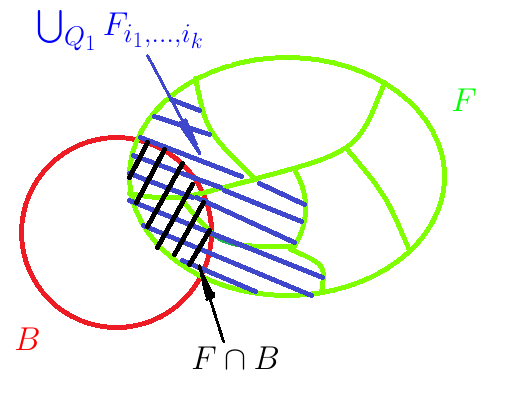
\includegraphics[width=4in]{fib}
  \caption{Rysunek wyjaśniający nierówność: $\tilde{\mu}(B)\leqslant \mu (\bigcup_{Q_1} I_{i_1,\ldots,i_k})$. Łatwo widać, że $F\cap B \subset \bigcup_{Q_1} F_{i_1,\ldots,i_k}$.}
\end{figure}

Tak więc: 

$\tilde{\mu}(B)\leqslant\sum_{Q_1}\mu(I_{i_1,\ldots,i_k}) = \sum_{Q_1} (c_{i_1}\ldots c_{i_k})^s \leqslant \sum_{Q_1} r^s \leqslant qr^s$

Ponieważ dowolny zbiór $U$ jest zawarty w kuli o promieniu $|U|$, wiemy, że:

$\tilde{\mu}(U)\leqslant|U|^sq$

Tak więc z tw. \eqref{mass} mamy: $\mathcal{H}^s(F)\geqslant \frac{1}{q}>0$ oraz $dim_HF\geqslant s$.

Czyli ostatecznie: $dim_HF = s$.

\end{dow}


%%%%%%%%%%%%%%%%%%%%%%%%%%%%%%%%%%przykłady%%%%%%%%%%%%%%%%%%%%%%%%%%%%%%%%%%%%%%%%%%%%%%%%%%%%%
\chapter{Przykłady}

W tym rozdziale przytoczę trzy przykłady zastosowania twierdzenia \ref{wym}. 

\section{Przykład 1.}

\begin{center}
\setlength{\unitlength}{0.7 mm}

\begin{picture}(100,100)

\put(0,0){\rule{200pt}{200pt}}

\end{picture}
\end{center}


\begin{center}
\setlength{\unitlength}{0.7 mm}

\begin{picture}(100,100)

\put(0,0){\line(0,1){100}}
\put(0,100){\line(1,0){100}}
\put(100,0){\line(0,1){100}}
\put(0,0){\line(1,0){100}}

\put(0,0){\rule{80pt}{80pt}}
\put(50,0){\rule{100pt}{100pt}}
\put(10,60){\rule{60pt}{60pt}}
\put(70,70){\rule{60pt}{60pt}}

\end{picture}
\end{center}


\begin{center}
\setlength{\unitlength}{0.7 mm}
\begin{picture}(100,100)

\put(0,0){\line(0,1){100}}
\put(0,100){\line(1,0){100}}
\put(100,0){\line(0,1){100}}
\put(0,0){\line(1,0){100}}

\put(50,0){\rule{40pt}{40pt}}
\put(75,0){\rule{50pt}{50pt}}
\put(55,30){\rule{30pt}{30pt}}
\put(85,35){\rule{30pt}{30pt}}

\put(0,0){\rule{32pt}{32pt}}
\put(20,0){\rule{40pt}{40pt}}
\put(28,28){\rule{24pt}{24pt}}
\put(4,24){\rule{24pt}{24pt}}

\end{picture}
\end{center}


%\begin{center}
%\setlength{\unitlength}{0.7 mm}

%\begin{picture}(100,100)
%\put(50,0){\line(0,1){50}}
%\put(50,50){\line(1,0){50}}

%\put(40,0){\line(0,1){40}}
%\put(0,40){\line(1,0){40}}

%\put(70,70){\line(0,1){30}}
%\put(70,70){\line(1,0){30}}

%\put(10,60){\line(0,1){30}}
%\put(10,60){\line(1,0){30}}
%\put(10,90){\line(1,0){30}}
%\put(40,60){\line(0,1){30}}
%\put(0,0){\rule{40pt}{40pt}}


%\color{blue}{\rule{1cm}{1cm}}
%\end{picture}
%\end{center}


\makestatement
\end{document}
